% !TEX TS-program = pdflatex
% !TEX encoding = UTF-8 Unicode

% This is a simple template for a LaTeX document using the "article" class.
% See "book", "report", "letter" for other types of document.

\documentclass[11pt]{article} % use larger type; default would be 10pt

\usepackage[utf8]{inputenc} % set input encoding (not needed with XeLaTeX)

%%% Examples of Article customizations
% These packages are optional, depending whether you want the features they provide.
% See the LaTeX Companion or other references for full information.

%%% PAGE DIMENSIONS
\usepackage{geometry} % to change the page dimensions
\geometry{a4paper} % or letterpaper (US) or a5paper or....
 \geometry{margin=1in} % for example, change the margins to 2 inches all round
% \geometry{landscape} % set up the page for landscape
%   read geometry.pdf for detailed page layout information

\usepackage{graphicx} % support the \includegraphics command and options

% \usepackage[parfill]{parskip} % Activate to begin paragraphs with an empty line rather than an indent

%%% PACKAGES
\usepackage{booktabs} % for much better looking tables
\usepackage{array} % for better arrays (eg matrices) in maths
\usepackage{paralist} % very flexible & customisable lists (eg. enumerate/itemize, etc.)
\usepackage{verbatim} % adds environment for commenting out blocks of text & for better verbatim
\usepackage{subfig} % make it possible to include more than one captioned figure/table in a single float
% These packages are all incorporated in the memoir class to one degree or another...

%%% HEADERS & FOOTERS
\usepackage{fancyhdr} % This should be set AFTER setting up the page geometry
\pagestyle{fancy} % options: empty , plain , fancy
\renewcommand{\headrulewidth}{0pt} % customise the layout...
\lhead{}\chead{}\rhead{}
\lfoot{}\cfoot{\thepage}\rfoot{}

%%% SECTION TITLE APPEARANCE
\usepackage{sectsty}
\allsectionsfont{\sffamily\mdseries\upshape} % (See the fntguide.pdf for font help)
% (This matches ConTeXt defaults)

%%% ToC (table of contents) APPEARANCE
\usepackage[nottoc,notlof,notlot]{tocbibind} % Put the bibliography in the ToC
\usepackage[titles,subfigure]{tocloft} % Alter the style of the Table of Contents
\renewcommand{\cftsecfont}{\rmfamily\mdseries\upshape}
\renewcommand{\cftsecpagefont}{\rmfamily\mdseries\upshape} % No bold!

%%% END Article customizations

%%% The "real" document content comes below...

\title{$4^{th}$ progress report}
%\author{The Author}
%\date{} % Activate to display a given date or no date (if empty),
         % otherwise the current date is printed 

\begin{document}
\maketitle
\section{Introduction}

 A first shareable version of the R code is included with this report. The code (described on last report) was implemented with: 
 
	\begin{itemize}
		\item A \verb|phyl()| function, which simulate a tree with rates generated by any of the three models described on next section of this report.
		\item An iterative method which estimate MLE values for a set of simulated trees.
 
	\end{itemize}
	
Moreover, the code generates the tree on Newick format as well for visual and topological analysis purposes. 


\section{Approach \& questions}


\subsection{Rates}

 We implement the model described on the previous reports, which considers the speciation and extinction rates as functions of traits depending on time $ \lambda_i = f(traits)$ and $\mu_i = f(traits)$. \\
  
 On this report we include two more models besides the loglinear, so we have the following three models:

\begin{itemize}
	\item[loglinear (Model 1):] 
 		$$\lambda_i = e^{\theta_0 + \theta_1 a_i} $$
		$$ \mu_i = e^{\varphi_0 + \varphi_1 a_i} $$
	\item[linear (Model 2):] 
		$$\lambda_i = \theta_0 + \theta_1 a_i $$
		$$ \mu_i = \varphi_0 + \varphi_1 a_i $$
	\item[logistic (Model 3):]
		$$\lambda_i = \frac{\theta_0}{1+e^{-\theta_1 a_i}}$$
\end{itemize}

\subsection{Questions:}

	\begin{itemize}
	%	\item Are those models realistic?, there is any bilogical meaning on this models? 
		\item Does the loglineal, linear and logistic models makes any biological sense?, It is ok to have same $f()$ for both, $\lambda$ and $\mu$?
		\item Would be a non-parametric approach a better alternative of those models?
		
		\item Why would we prefer this framework instead of the differential approach of Nee et al. ?
	

	\end{itemize}



\section{Implementation}


\subsection{Simulation}

We use the \verb|phyl()| function to simulate trees, an exaple of a 10-iteration phylogenetic tree would be:  
	\begin{verbatim}
	s1 = phyl(nT=10, model = "loglinear")
	\end{verbatim}

	 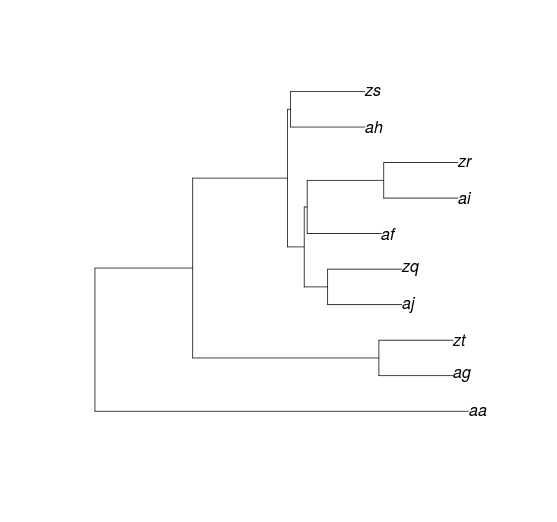
\includegraphics[scale=0.5]{phylo.png}

We simulated 1000 different trees with same parametes and we estimated it using MLE. A summary of the estimated values for each model is described included bellow. In general we have similar results given in the last report. 


\begin{table}[ht]
\centering
\begin{tabular}{rrrrrrr}
  \hline
 & n & real value & mean & median & min & max \\ 
  \hline
1 & 1000 & 3.00 & 3.00 & 2.98 & 0.62 & 5.81 \\ 
  2 & 1000 & 4.00 & 5.03 & 3.95 & -591.87 & 2410.71 \\ 
  3 & 1000 & 1.00 & 1.56 & 0.87 & -13.42 & 347.45 \\ 
  4 & 1000 & 2.00 & -1.03 & 1.63 & -4045.67 & 2003.04 \\ 
   \hline
\end{tabular}
\caption{Model 1}
\end{table}

% latex table generated in R 3.2.1 by xtable 1.8-0 package
% Fri Jan 29 18:52:08 2016
\begin{table}[ht]
\centering
\begin{tabular}{rrrrrrr}
  \hline
 & n & real value & mean & median & min & max \\ 
  \hline
1 & 1000.00 & 3.00 & 2.83 & 2.85 & -15.46 & 17.76 \\ 
  2 & 1000.00 & 4.00 & 13.43 & 3.87 & -4131.72 & 3329.81 \\ 
  3 & 1000.00 & 1.00 & 1.02 & 0.94 & -15.02 & 18.60 \\ 
  4 & 1000.00 & 2.00 & -5.88 & 1.60 & -7333.90 & 3473.38 \\ 
   \hline
\end{tabular}
\caption{Model 2}
\end{table}


% latex table generated in R 3.2.1 by xtable 1.8-0 package
% Fri Jan 29 18:48:56 2016
\begin{table}[ht]
\centering
\begin{tabular}{rrrrrrr}
  \hline
 & n & real value & mean & median & min & max \\ 
  \hline
1 & 1000.00 & 3.00 & 4.55 & 3.34 & 1.39 & 63.37 \\ 
  2 & 1000.00 & 4.00 & 10.09 & 2.02 & -1118.53 & 2702.20 \\ 
  3 & 1000.00 & 1.00 & 2.64 & 1.07 & 0.34 & 180.18 \\ 
  4 & 1000.00 & 2.00 & -0.75 & 1.46 & -3027.31 & 2999.15 \\ 
   \hline
\end{tabular}
\caption{Model 3}
\end{table}
\newpage
\subsection{Analysis}

Some visual analysis tools are also provided with the code, we used them to find relationships between "bad" estimations and both, numerical and topological data. 

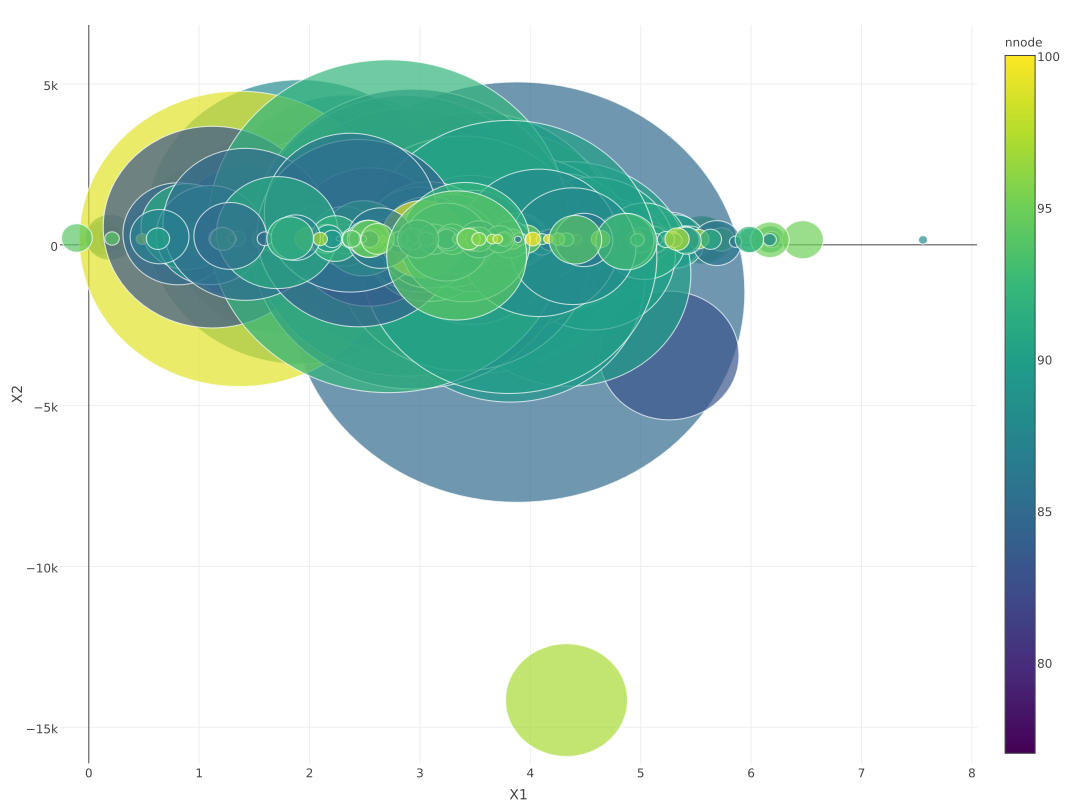
\includegraphics[scale=0.3]{vis.png}

After comparison we found no relationship betwen particular caracteristics of the trees and non accurate estimations.

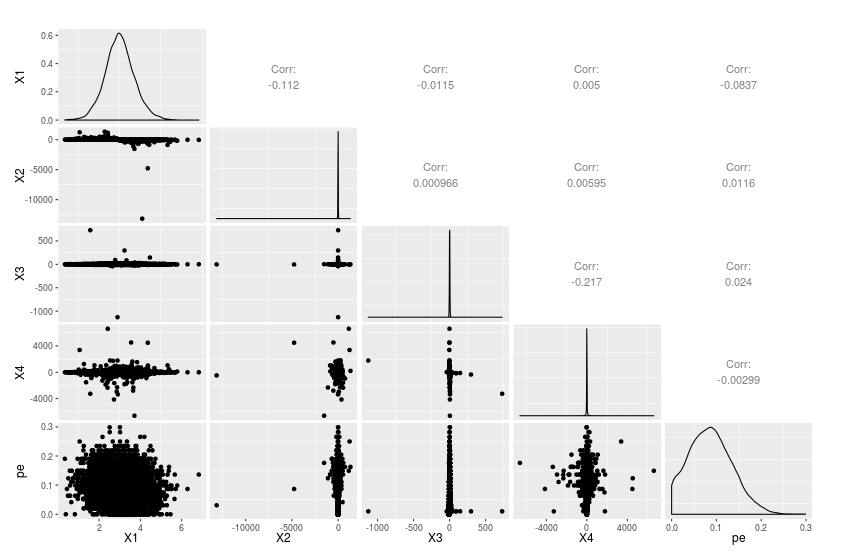
\includegraphics[scale=0.5]{pairs}

%\section{First section}
%
%
%
%
%
%\subsection{A subsection}
%
%% latex table generated in R 3.2.1 by xtable 1.8-0 package
%% Fri Jan 29 19:08:18 2016
%\begin{table}[ht]
%\centering
%\begin{tabular}{rrrrrrr}
%  \hline
% & n & real value & mean & median & min & max \\ 
%  \hline
%1 & 10000.00 & 3.00 & 3.02 & 3.00 & 0.02 & 6.27 \\ 
%  2 & 10000.00 & 4.00 & 2.92 & 3.88 & -5344.38 & 8316.81 \\ 
%  3 & 10000.00 & 1.00 & 1.30 & 0.89 & -85.51 & 1730.75 \\ 
%  4 & 10000.00 & 2.00 & 0.33 & 1.41 & -14784.51 & 6445.60 \\ 
%   \hline
%\end{tabular}
%\caption{Model 1}
%\end{table}
%
%
%More text.

\end{document}